%!TEX root = ../Touch Based Idris.tex
\appendix
\label{Appendix}
\chapter{Running The Code}
\label{chap:RunningTheCode}
The final revision of the iPad prototype and the server code are available at
Github: 
\paragraph{Repo address:} \url{https://github.com/nicolaidahl/touchbasedidris}
\paragraph{Final git revision:} 535683bd48973a6ab41a0a96d447d50a18cfe711
\paragraph{}
Running the iPad prototype in a simulator requires a Mac with Xcode installed. Furthermore,
Cocoapods is required for dependency management. Get it here: \url{http://cocoapods.org/}

To run the iPad prototype: 
\begin{enumerate}
	\item Navigate to /src and run \texttt{pod install}
	\item Open the IdrisTouch.xcworkspace file that just appeared
	\item Make sure that the upper left-hand side of Xcode says ``IdrisTouch -> iPad
	Retina (64-bit)''
	\item Hit Cmd+R to run the prototype
\end{enumerate}

Please note that the app is still unstable and that it has only been developed
to the point where it sufficed for the second usability test.

\chapter{First Usability Test}
\label{chap:FirstUsabilityTest}
%!TEX root = ../../Touch Based Idris.tex 

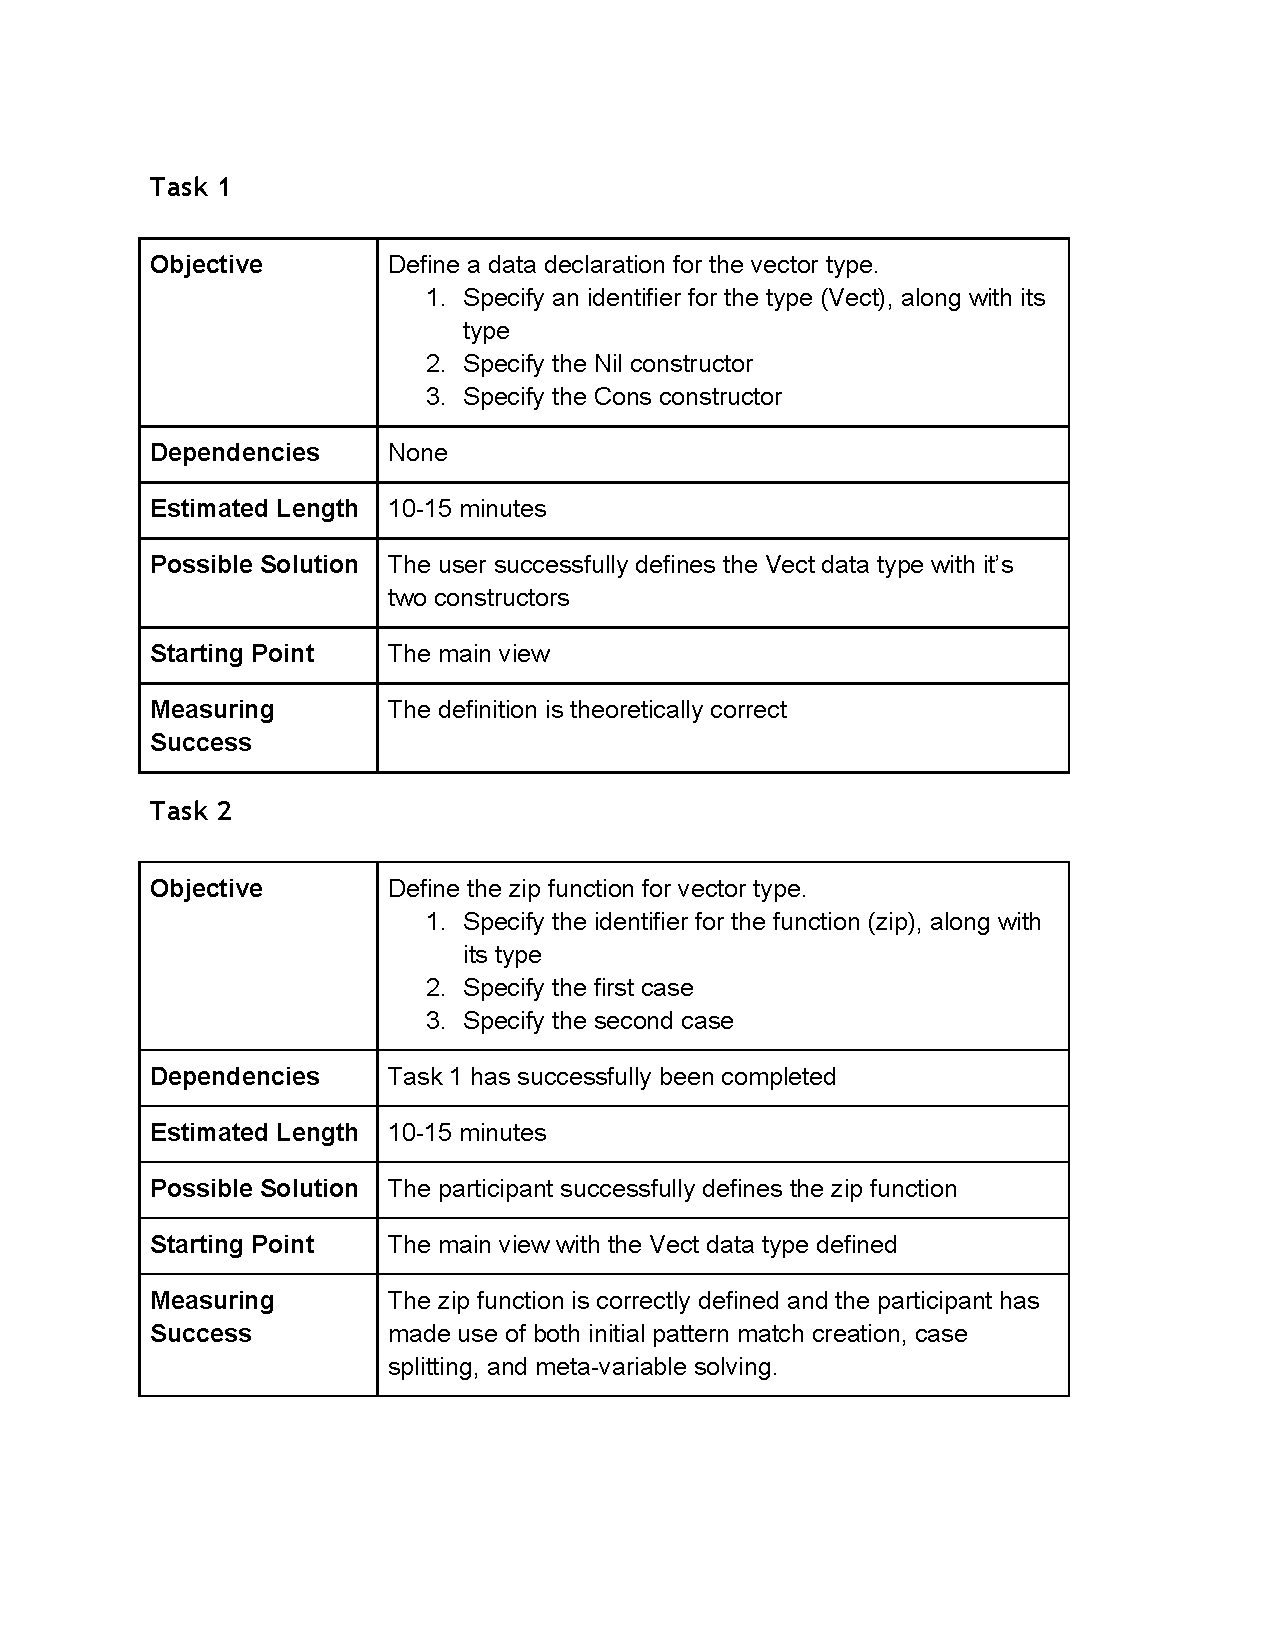
\includegraphics[width=150mm]{sections/appendix/FirstUsabilityTestFormal.pdf}

\chapter{Second Usability Test}
\label{chap:SecondUsabilityTest}
%!TEX root = ../../Touch Based Idris.tex 

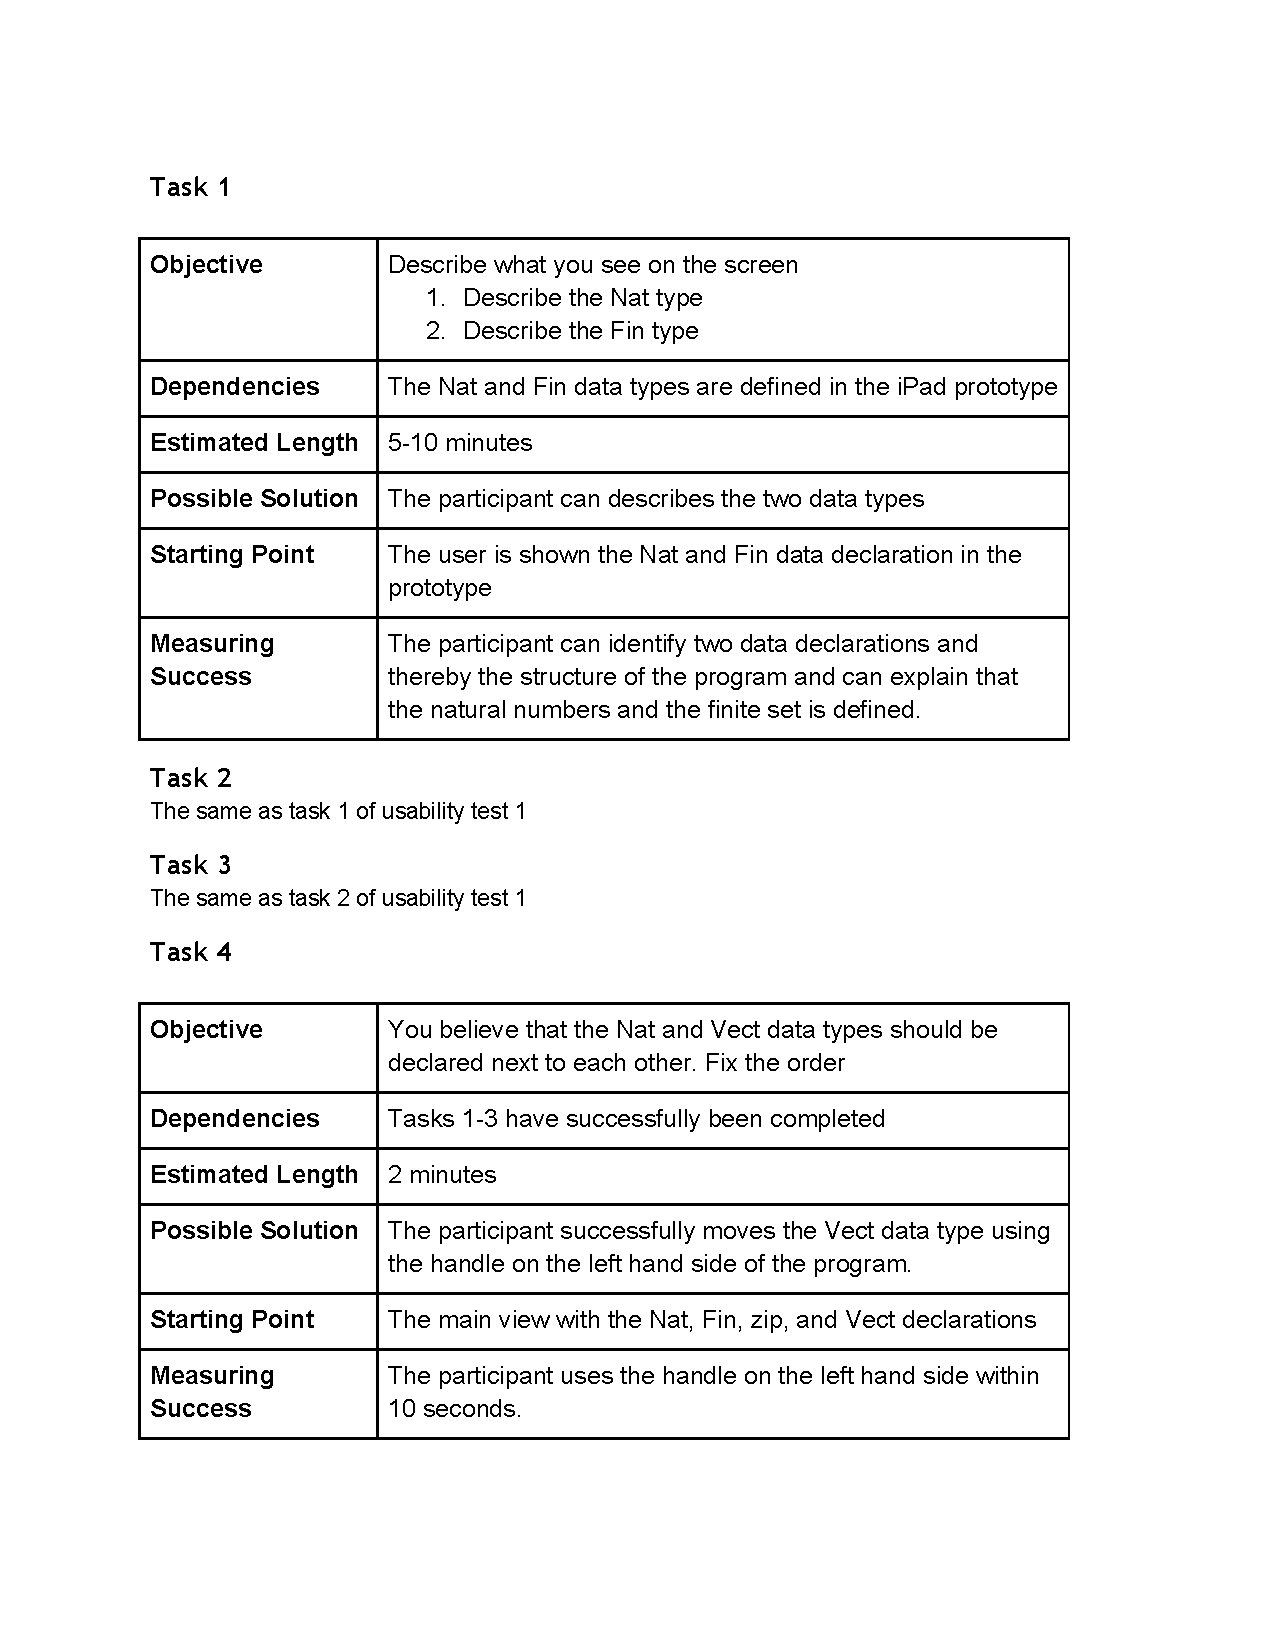
\includegraphics[width=150mm]{sections/appendix/SecondUsabilityTestFormal.pdf}

\chapter{IdrisTouch AST}
\label{chap:IdrisTouch_AST}

\lstinputlisting[language=Haskell, firstline=0]{code/IdrisTouchAST.hs}

\chapter{All Takeaways}
\label{chap:AllTakeaways}
%!TEX root = ../../Touch Based Idris.tex 
A list of all takeaways from Chapter~\ref{sec:Analysis}.
\begin{itemize}
	\item \textbf{Ta-1}: Do not assume that a virtual keyboard is as usable as a physical one\,\cite{nielsen2013mobile}. The touch interface has potential if you design your user experience to take advantage of it, but if you chose to ignore its potential/limitations you will have lower usability\,\cite{nielsen1990heuristic}.
	\item \textbf{Ta-2}: You need accelerators for users to become faster and more comfortable with the interface\,\cite{nielsen1990heuristic}. An accelerator could, for example, be auto completion and/or static checking.
	\item \textbf{Ta-3}: Undo support is essential for usability\,\cite{nielsen1990heuristic}, but shaking the device is probably not the right input method.
	\item \textbf{Ta-4}: The solution Textastic has come up with for quickly accessing a large collection of symbols is the most intuitive we have seen.
	\item \textbf{Ta-5}: It is not enough to have a good editing interface, if such a basic issue as running your code is unaddressed.
		\item \textbf{Ta-6}: A good edit-compile-test loop greatly improves the development flow.
	\item \textbf{Ta-7}: A solid way to recover from syntax errors is essential to a good development experience\,\cite{nielsen1990heuristic}.
	\item \textbf{Ta-8}: The error messages from the compiler/interpreter should indicate where in the code the syntax errors have occurred. Simply presenting ``Unknown Error'' is frustrating for the user.
	\item \textbf{Ta-9}: It should not be necessary to add a PDF document with instructions to how the gestures and buttons work. It should be immediately recognized by the user because it is all presented according to the platform standards. This serves as a reminder that the overuse of clever gestures harms the user experience.
	\item \textbf{Ta-10}: Littering a structured editor with [+] (add) buttons, to indicate that expressions can be added at these positions, is not a good idea. While a good alternative for this solution is hard to come up with we should try to design a different way.
	\item \textbf{Ta-11}: Having a popup close to the goal makes for quick and easy access. The better that popup is at guessing the right thing for the goal, the faster the tool will seem.
	\item \textbf{Ta-12}: Eastwest is a good indication that functional languages work well in a structured editor.
	\item \textbf{Ta-13}: To have a contextual overview can speed up the tasks of programming just as we saw with Eastwest.
	\item \textbf{Ta-14}: The type system of the TouchDevelop object oriented programming language is not ideal if you want to expose a context for the user to pick from. The type system simply can't narrow down the possibilities efficiently.
	\item \textbf{Ta-15}: Using a smaller font for code that is not in focus is a clever way to create a better overview for the user.
	\item \textbf{Ta-16}: There is a clear difference between the feel of a web app like TouchDevelop and a native app like Lisping.
	\item \textbf{Ta-17}: One interpretation of Whitley and Blackwell's findings\,\cite{WHITLEY2001435} is that although LabVIEW can be hard for programmers not used to the visual syntax, the higher learning curve pays off in the long run.
	\item \textbf{Ta-18}: The ``boxes and wires'' approach is good at indicating structure and could maybe be transfered to a more general purpose language.
	\item \textbf{Ta-19}: When designing a visual syntax, making it visually obvious which elements go together greatly increases the ease of learning.
	\item \textbf{Ta-20}: Using colors and shapes to differentiate elements is very important in a visual language.
	\item \textbf{Ta-21} Complexity management is hard with visual languages\,\cite{green1992visual}.
	\item \textbf{Ta-22}: Use all the aspects of visual expressiveness when designing a visual language, e.g.\ shape, color, texture, position, etc.
	\item \textbf{Ta-23}: The more visual way of writing data types could be more intuitive for people used to reading that sort of notation. This goes well with Nielsen’s ``Match between system and the real world''-heuristic.
\end{itemize}


\chapter{List of Goals and Requirements}
\label{chap:ListOfAllGoalsAndRequirements}
%!TEX root = ../../Touch Based Idris.tex 

\paragraph{Goals}
The high-level goals of the project:

\begin{itemize} 
	\item \textbf{G-1}: To design a programming editor that leverages Idris to provide a usable solution for the touch-based iPad device
	(Ta-12).
	\item \textbf{G-2}: The edit-compile-test cycle should be as fast as state of the art iPad programming editors
	(Ta-6, Ta-12).
	\item \textbf{G-3}: Minimize the use of the virtual keyboard\,\cite[pp. 76]{nielsen2013mobile} and ideally only make use of it when inputting identifiers or auto completing terms
	(Ta-1, Ta-11, Ta-12).
	\item \textbf{G-4}: The solution should be eligible for submission to the Apple App Store (Ta-5). 
\end{itemize}

\paragraph{Usability Requirements}

The interface should:
\begin{itemize}     
	\item \textbf{U-1}: Clearly communicate program structure. One way to accomplish this it through the use of visual elements such as shape, color and connecting lines (G-1)
	(Ta-18, Ta-19, Ta-20, Ta-22).
	\item \textbf{U-2}: Make use of touch gestures only when it can improve usability (G-1)
	(Ta-2, Ta-9).
	\item \textbf{U-3}: If using visual elements, avoid the pitfall of some visual languages\,\cite{green1992visual} and ensure that the program structure approximately scales to the same degree as state of the art touch-based editors (G-1)
	(Ta-17, Ta-21).
	\item \textbf{U-4}: Implement accelerators for use by the expert user but invisible for the novice user\,\cite{nielsen1990heuristic}, preferably by use of simple touch gestures (G-1, G-2, G-3)
	(Ta-1, Ta-2, Ta-4).
	\item \textbf{U-5}: Allow the user to recover from syntactical as well as logical errors in a fast manner (G-2)
	(Ta-3, Ta-6, Ta-7, Ta-8).
	\item \textbf{U-6}: Have a clear indication of where the user can add and edit terms without these indications cluttering the interface (see Section~\ref{subsub:Lisping}) (G-1)
	(Ta-10).
\end{itemize}

\paragraph{Functional Requirements}

Specifically the design must:

\begin{itemize}
	\item \textbf{F-1}: Support initial pattern match creation like the Idris Emacs mode\,\cite{Idris:EmacsMode} (G-1, G-2, G-3)
	(Ta-1, Ta-2).
	\item \textbf{F-2}: Support case splitting of pattern variables like the Emacs mode\,\cite{Idris:EmacsMode} (G-1, G-2, G-3) (Ta-1, Ta-2).
	\item \textbf{F-3}: Support a way to let Idris automatically solve a metavariable like the Emacs mode\,\cite{Idris:EmacsMode} (G-1, G-2, G-3) (Ta-1, Ta-2).
	\item \textbf{F-4}: Allow the user to add, remove, and edit basic data types like \texttt{Vect} (G-1).
	\item \textbf{F-5}: Allow the user to add, remove, and edit basic functions like the \texttt{zip} function (G-1).
	\item \textbf{F-6}: Comply with the Apple App Store Review Guidelines\,\cite{AppStoreGuidelines} (G-4)
	(Ta-5).
	\item \textbf{F-7}: Include an overview of the possible language constructs that are applicable in the current context, inspired by TouchDevelop (see Section~\ref{subsub:TouchDevelop}), Lisping (see Section~\ref{subsub:Lisping}), and Eastwest (see Section~\ref{subsub:Eastwest}) (G-1, G-2, G-3)
	(Ta-11, Ta-12, Ta-13, Ta-14).
	\item \textbf{F-8}: Provide better undo support than simply shaking the device (see Section~\ref{subsub:CodeToGo}) (G-2)
	(Ta-3).
	\item \textbf{F-9}: Collapse or minimize top level declarations not currently in focus. This is inspired by TouchDevelop (see Section~\ref{subsub:TouchDevelop}) (G-2, U-3)
	(Ta-15).
	\item \textbf{F-10}: Allow for a faster way of accessing special characters (see Section~\ref{subsub:Textastic}) (G-2)
	(Ta-4).
\end{itemize}